% This work is licensed under the Creative Commons
% Attribution-NonCommercial-ShareAlike 4.0 International License. To view a copy
% of this license, visit http://creativecommons.org/licenses/by-nc-sa/4.0/ or
% send a letter to Creative Commons, PO Box 1866, Mountain View, CA 94042, USA.

\documentclass[12pt,a4paper]{article} 

% This work is licensed under the Creative Commons
% Attribution-NonCommercial-ShareAlike 4.0 International License. To view a copy
% of this license, visit http://creativecommons.org/licenses/by-nc-sa/4.0/ or
% send a letter to Creative Commons, PO Box 1866, Mountain View, CA 94042, USA.

% PACKAGES
\usepackage[english, ngerman]{babel}	% Paket für Sprachselektion, in diesem Fall für deutsches Datum etc
\usepackage[utf8]{inputenc}	% Paket für Umlaute; verwende utf8 Kodierung in TexWorks 
\usepackage[T1]{fontenc} % ö,ü,ä werden richtig kodiert
\usepackage{amsmath} % wichtig für align-Umgebung
\usepackage{amssymb} % wichtig für \mathbb{} usw.
\usepackage{amsthm} % damit kann man eigene Theorem-Umgebungen definieren, proof-Umgebungen, etc.
\usepackage{mathrsfs} % für \mathscr
\usepackage[backref]{hyperref} % Inhaltsverzeichnis und \ref-Befehle werden in der PDF-klickbar
\usepackage[english, ngerman, capitalise]{cleveref}
\usepackage{graphicx}
\usepackage{grffile}
\usepackage{setspace} % wichtig für Lesbarkeit. Schöne Zeilenabstände

\usepackage{enumitem} % für custom Liste mit default Buchstaben
\usepackage{ulem} % für bessere Unterstreichung
\usepackage{contour} % für bessere Unterstreichung
\usepackage{epigraph} % für das coole Zitat

\usepackage{tikz}

% This work is licensed under the Creative Commons
% Attribution-NonCommercial-ShareAlike 4.0 International License. To view a copy
% of this license, visit http://creativecommons.org/licenses/by-nc-sa/4.0/ or
% send a letter to Creative Commons, PO Box 1866, Mountain View, CA 94042, USA.

% THEOREM-ENVIRONMENTS

\newtheoremstyle{mystyle}
  {20pt}   % ABOVESPACE \topsep is default, 20pt looks nice
  {20pt}   % BELOWSPACE \topsep is default, 20pt looks nice
  {\normalfont} % BODYFONT
  {0pt}       % INDENT (empty value is the same as 0pt)
  {\bfseries} % HEADFONT
  {}          % HEADPUNCT (if needed)
  {5pt plus 1pt minus 1pt} % HEADSPACE
	{}          % CUSTOM-HEAD-SPEC
\theoremstyle{mystyle}

% Definitionen der Satz, Lemma... - Umgebungen. Der Zähler von "satz" ist dem "section"-Zähler untergeordnet, alle weiteren Umgebungen bedienen sich des satz-Zählers.
\newtheorem{satz}{Satz}[section]
\newtheorem{lemma}[satz]{Lemma}
\newtheorem{korollar}[satz]{Korollar}
\newtheorem{proposition}[satz]{Proposition}
\newtheorem{beispiel}[satz]{Beispiel}
\newtheorem{definition}[satz]{Definition}
\newtheorem{bemerkungnr}[satz]{Bemerkung}
\newtheorem{theorem}[satz]{Theorem}

% Bemerkungen, Erinnerungen und Notationshinweise werden ohne Numerierungen dargestellt.
\newtheorem*{bemerkung}{Bemerkung.}
\newtheorem*{erinnerung}{Erinnerung.}
\newtheorem*{notation}{Notation.}
\newtheorem*{aufgabe}{Aufgabe.}
\newtheorem*{lösung}{Lösung.}
\newtheorem*{beisp}{Beispiel.} %Beispiel ohne Nummerierung
\newtheorem*{defi}{Definition.} %Definition ohne Nummerierung
\newtheorem*{lem}{Lemma.} %Lemma ohne Nummerierung


% SHORTCUTS
\newcommand{\R}{\mathbb{R}}				 % reelle Zahlen
\newcommand{\Rn}{\R^n}						 % der R^n
\newcommand{\N}{\mathbb{N}}				 % natürliche Zahlen
\newcommand{\Z}{\mathbb{Z}}				 % ganze Zahlen
\newcommand{\C}{\mathbb{C}}			   % komplexe Zahlen
\newcommand{\gdw}{\Leftrightarrow} % Genau dann, wenn
\newcommand{\with}{\text{ mit }}   % mit
\newcommand{\falls}{\text{falls }} % falls
\newcommand{\dd}{\text{ d}}        % Differential d

% ETWAS SPEZIELLERE ZEICHEN
%disjoint union
\newcommand{\bigcupdot}{
	\mathop{\vphantom{\bigcup}\mathpalette\setbigcupdot\cdot}\displaylimits
}
\newcommand{\setbigcupdot}[2]{\ooalign{\hfil$#1\bigcup$\hfil\cr\hfil$#2$\hfil\cr\cr}}
%big times
\newcommand*{\bigtimes}{\mathop{\raisebox{-.5ex}{\hbox{\huge{$\times$}}}}} 

% WHITESPACE COMMANDS
%non-restrict newline command
\newcommand{\enter}{$ $\newline} 
%praktischer Tabulator
\newcommand\tab[1][1cm]{\hspace*{#1}}

% TEXT ÜBER ZEICHEN
%das ist ein Gleichheitszeichen mit Text darüber, Beispiel: $a\stackeq{Def} b$
\newcommand{\stackeq}[1]{
	\mathrel{\stackrel{\makebox[0pt]{\mbox{\normalfont\tiny #1}}}{=}}
} 
%das ist ein beliebiges Zeichen mit Text darüber, z. B.  $a\stackrel{Def}{\Rightarrow} b$
\newcommand{\stacksymbol}[2]{
	\mathrel{\stackrel{\makebox[0pt]{\mbox{\normalfont\tiny #1}}}{#2}}
} 

% UNDERLINE
% besseres underline 
\renewcommand{\ULdepth}{1pt}
\contourlength{0.5pt}
\newcommand{\ul}[1]{
	\uline{\phantom{#1}}\llap{\contour{white}{#1}}
}


% hier noch ein paar Commands die nur ich nutze, weil ich sie mir im Laufe der Jahre angewöhnt habe und sie mir jetzt nicht abgewöhnen will:

\newcommand{\gdw}{\Leftrightarrow}   % genau dann, wenn




\author{Willi Sontopski}

\parindent0cm %Ist wichtig, um führende Leerzeichen zu entfernen

\usepackage{pdflscape}
\usepackage{rotating}
\usepackage{scrpage2}
\pagestyle{scrheadings}
\clearscrheadfoot

\ihead{Willi Sontopski}
\chead{Formale Systeme WiSe 18 19}
\ohead{}
\ifoot{Blatt 10}
\cfoot{Version: \today}
\ofoot{Seite \pagemark}

\newcommand{\A}{\mathcal{A}}

\begin{document}
%\setcounter{section}{1}

\section*{Aufgabe $\ast$)}
Gegeben ist der $\varepsilon$-NEA
\begin{align*}
	\A=\Big(\lbrace q_0,\ldots,q_4\rbrace,\lbrace a,b\rbrace,q_0,\Delta,\lbrace q_2\rbrace\Big)
\end{align*}

\usetikzlibrary{positioning,automata}
\begin{tikzpicture}[shorten >=1pt,node distance=2.7cm,on grid]
  \node[state,initial]   	(q_0)                		{$q_0$};
  \node[state] 				(q_1) [above right=of q_0] 	{$q_1$};
  \node[state, accepting] 	(q_2) [right=of q_1] 		{$q_2$};
  \node[state] 				(q_3) [below right=of q_0] 	{$q_3$};
  \node[state] 				(q_4) [right=of q_3]		{$q_4$};
  \path[->] (q_0) edge [bend left=0] node [above] {a} (q_1)
                  edge [bend left=0] node [above] {b} (q_3)
            (q_1) edge [bend left=0] node [above] {$\varepsilon$} (q_2)
            	  edge [bend left=0] node [left] {a,b} (q_3)
            (q_2) edge [bend left=0] node [right] {a} (q_3)
                  edge [bend left=0] node [right] {a} (q_4)
            (q_3) edge [bend left=0] node [above] {b} (q_4)
            (q_4) edge [loop right] node [right] {a} ();
\end{tikzpicture}

Zuerst entfernen wir die $\varepsilon$-Transitionen auf naheliegende Weise:

\usetikzlibrary{positioning,automata}
\begin{tikzpicture}[shorten >=1pt,node distance=2.7cm,on grid]
  \node[state,initial]   	(q_0)                		{$q_0$};
  \node[state] 				(q_1) [above right=of q_0] 	{$q_1$};
  \node[state, accepting] 	(q_2) [right=of q_1] 		{$q_2$};
  \node[state] 				(q_3) [below right=of q_0] 	{$q_3$};
  \node[state, accepting] 				(q_4) [right=of q_3]		{$q_4$};
  \path[->] (q_0) edge [bend left=0] node [above] {a} (q_1)
                  edge [bend left=0] node [above] {b} (q_3)
            (q_1) edge [bend left=0] node [above] {a} (q_4) %Diese Transition wurde geändert
            	  edge [bend left=0] node [left] {a,b} (q_3)
            (q_2) edge [bend left=0] node [right] {a} (q_3)
                  edge [bend left=0] node [right] {a} (q_4)
            (q_3) edge [bend left=0] node [above] {b} (q_4)
            (q_4) edge [loop right] node [right] {a} ();
\end{tikzpicture}

Wichtig ist hierbei, dass nun $q_4$ auch ein Endzustand geworden ist.
Nun erzeugen wir den äquivalenten DEA mithilfe der Potenzmengenkonstruktion:

\usetikzlibrary{positioning,automata}
\begin{tikzpicture}[shorten >=1pt,node distance=2.7cm,on grid]
  \node[state,initial]   	(q_0)                		{$\lbrace q_0\rbrace$};
  \node[state] 				(q_1) [above right=of q_0] 	{$\lbrace q_1\rbrace$};
  \node[state, accepting] 	(q_3q_4) [right=of q_1] 		{$\lbrace q_3,q_4\rbrace$};
  \node[state] 				(q_3) [below right=of q_0] 	{$\lbrace q_3\rbrace$};
  \node[state, accepting] 	(q_4) [right=of q_3]		{$q_4$};
  \node[state]				(T)	  [below right =of q_3q_4] {$\emptyset$};
  \path[->] (q_0) edge [bend left=0] node [above] {a} (q_1)
                  edge [bend left=0] node [above] {b} (q_3)
            (q_1) edge [bend left=0] node [above] {a} (q_3q_4)
            	  edge [bend left=0] node [left] {b} (q_3)
            (q_3q_4) edge [bend left=0] node [right] {a,b} (T)
                  %edge [bend left=0] node [right] {a} (q_4)
            (q_3) edge [bend left=0] node [above] {b} (q_4)
            	  edge [bend left=30] node [below] {a} (T)
            (q_4) edge [loop right] node [right] {a} ()
            	  edge [bend left=0] node [below] {b} (T)
           	(T)   edge [loop right] node [above] {a,b} ();
\end{tikzpicture}

Den unerreichbaren Zustand $q_2$ braucht man nicht beachten. Den Papierkorbzustand $\emptyset$ nicht vergessen. Also ist der äquivalente DEA:
\begin{align*}
	\A'&=\Big(\big\lbrace q_0\rbrace,\lbrace q_1\rbrace,\lbrace q_3\rbrace,\lbrace q_3,q_4\rbrace,\lbrace q_4\rbrace,\emptyset\big\rbrace,\lbrace a,b\rbrace,\lbrace q_0\rbrace,\delta,\big\lbrace\lbrace q_3,q_4\rbrace,\lbrace q_4\rbrace\big\rbrace\Big)\\
	\overset{\text{Umbennung}}&{=:}
	\Big(\underbrace{\lbrace p_0, p_1,p_3,p_2,p_4, p_5\rbrace}_{=:P},\lbrace a,b\rbrace,p_0,\delta,\lbrace p_2,p_4\rbrace\Big)
\end{align*}

Da $\A'$ keine unerreichbaren Zustände mehr besitzt, gilt $\A_0=\A'$.
Um $\A_{\text{red}}$ zu berechnen, berechnen wir $\sim_{\A}$ schrittweise durch $\sim_k$:
\begin{itemize}
	\item $P|_{\sim_0}=\big\lbrace\lbrace p_2,p_4\rbrace,\lbrace p_0,p_1,p_3,p_5\rbrace\big\rbrace$ (Startzustände und Endzustände trennen)
	\item $P|_{\sim_1}=\big\lbrace\lbrace p_2\rbrace,\lbrace p_4\rbrace,\lbrace p_0, p_5\rbrace,\lbrace p_1\rbrace,\lbrace p_3\rbrace\big\rbrace$
	\item $P|_{\sim_2}=\big\lbrace\lbrace p_2\rbrace,\lbrace p_4\rbrace,\lbrace p_0\rbrace,\lbrace p_5\rbrace,\lbrace p_1\rbrace,\lbrace p_3\rbrace\big\rbrace$
\end{itemize}
Es gilt also $\sim_3=\sim_2\implies\sim_\A=\sim_2$. 
Da hier alle Zustände paarweise nicht äquivalent zueinander sind, gilt:
\begin{align*}
	\A_{\text{red}}=\tilde{\A_0}\cong\A_0=\A'
\end{align*}

\section*{Aufgabe 1}
Meine Idee (geht sicher viel eleganter):\\
Da es sehr viele Zerlegungsmöglichkeiten pro Wort $w$ gibt, ist es geschickter zu schauen, für welche $y\in\Sigma^+$ überhaupt die Eigenschaft 
\begin{align*}
	\exists x,z\in\Sigma^\ast:\forall k\in\N:xy^kz\in L(\A)
\end{align*}
gilt.
Man sieht, dass nur $y\in\lbrace c,cd,dc\rbrace=:M$ dies erfüllen. Nun gehen wir $w$ einzeln durch und schauen uns nur die Zerlegungen an, bei der $y\in M$ gilt (denn nur die sind interessant). Da $x,z=\varepsilon$ möglich, erhalten wir genau diese möglichen Zerlegungen durch \textit{Stringvergleich}, d.h. wir schauen, ob ein $p\in M$ existiert, welches ein Substring von dem festen $w$ ist. Also: (Nutze Kurzschreibweise $\alpha|\beta|\gamma$ für Zerlegung des Wortes $w$ in $x=\alpha$, $y=\beta$ und $z=\gamma$)
\begin{itemize}
	\item $w=adc$: Mögliche Zerlegungen: 
	\begin{itemize}
		\item $\varepsilon|c|da$: ist nicht in $L(\A)$.
		\item $a|cd$: ist in $L(\A)$ und erfüllt \eqref{eqAufgabe1} fast, jedoch nur für $k>1$.
	\end{itemize}
	\item $w=cda$ ist gar nicht in $L(\A)$, weshalb keine solche Zerlegungen existieren können, die \eqref{eqAufgabe1} erfüllen. 
	\item $w=bcdc$ Mögliche Zerlegungen: 
	\begin{itemize}
		\item $b|c|dc$: erfüllt \eqref{eqAufgabe1}.
		\item $bcd|c|\varepsilon$: erfüllt \eqref{eqAufgabe1} nicht, da $c$ nicht mehr "geloopt" werden kann, nach $acd$ gelesen wurde.
		\item $b|cd|c$: erfüllt \eqref{eqAufgabe1}.
		\item $bc|dc|\varepsilon$: erfüllt \eqref{eqAufgabe1}.
	\end{itemize}
	\item $acdc$ Mögliche Zerlegungen: 
	\begin{itemize}
		\item $a|c|dc$: erfüllt \eqref{eqAufgabe1}.
		\item $acd|c|\varepsilon$ erfüllt \eqref{eqAufgabe1} nicht, da $c$ dann nicht mehr geloopt werden kann.
		\item $ac|dc|\varepsilon$ erfüllt \eqref{eqAufgabe1}.
		\item $a|cd|c$ erfüllt \eqref{eqAufgabe1}.
	\end{itemize}
\end{itemize}
Somit erhalten wir für $adc$ 0, für $cda$ 0, für $bcdc$ 3 und für $acdc$ 3 Zerlegungen, die die gesuchten Eigenschaft erfüllen:

\begin{align}\label{eqAufgabe1}
	\forall k\in\N:xy^kz\in L(\A)
\end{align}

\section*{Aufgabe 2}
Die Sprache
\begin{align*}
	L:=\big\lbrace a^p\mid p\text{ ist Primzahl}\big\rbrace\mit\Sigma:=\lbrace a\rbrace
\end{align*}
ist nicht erkennbar.

\begin{proof}
	Wir führen einen Widerspruchsbeweis: Angenommen, $L$ ist erkennbar.
	Dann folgt aus dem Pumping-Lemma (3.1): Es gibt $n_0\in\N_{\geq1}$ so, dass jedes Wort $w\in L$ mit $|w|\geq n_0$ sich zerlegen lässt in $w=xyz$ mit $y\neq\varepsilon$ und $xy^kz\in L$ für alle $k\geq0$.
	Sei also $w=a\ldots a\in L$ beliebig mit $p\geq n_0$. Also gilt
	\begin{align*}
		&w=\underbrace{a\ldots a}_{p\geq n_0\text{ Stück}}\overset{!}= xy^k z\\
		&\implies \exists l,m,n\in\N_{\geq0}: w=a^p=a^l a^m a^n\\
		&\implies p=l+m+n
	\end{align*}
	Nach Voraussetzung ist $p$ eine Primzahl und nach Pumpinglemma gilt:
	\begin{align*}
		&x y^k z\in L &\forall k\in\N_{\geq0}\\
		&\implies l+m\cdot k+ n\text{ ist Primzahl} &\forall k\in\N_{\geq0}
	\end{align*}
	Dies ist aber im Allgemeinen keine Primzahl (was ich gerade leider nicht für alle Fälle zeigen kann...).\\
	Widerspruch! Somit ist $L$ nicht erkennbar.
\end{proof}

\section*{Aufgabe 3}
Die Sprache
\begin{align*}
	L:=\Big\lbrace w\mid w=1^k\text{ für }k\geq0\text{ oder }w=0^j1^p\text{ für }j\geq1\text{ und }p\text{ Primzahl}\Big\rbrace\\
	\mit\Sigma=\lbrace0,1\rbrace
\end{align*}
ist nicht erkennbar.

\begin{proof}
	%TODO
\end{proof}

\section*{Aufgabe 4}
\textbf{Satz 4.1} Ist $L$ erkennbar, so ist auch $L^\ast$ erkennbar.

\begin{proof}
	%Erinnerung: Eine Sprache $L$ ist per Definition erkennbar, wenn es einen NEA $\A$ gibt, der $L$ akzeptiert, d.a. $L=L(\A)$.\nl
	Da $L$ erkennbar ist, gibt es per Definition einen NEA
	\begin{align*}
		\A:=(Q,\Sigma,q_0,\Delta,F)
	\end{align*}
	mit $L(\A)=L$. 
	Sei nun $q_{0\varepsilon}\not\in Q$ und setze
	\begin{align*}
		\A_\varepsilon&:=\Big(Q\cup\lbrace q_{0\varepsilon}\rbrace,\Sigma,q_{0\varepsilon},\Delta_\varepsilon,\lbrace q_{0\varepsilon}\rbrace\Big)\\
		\Delta_\varepsilon&:=\Delta\cup\underbrace{\big\lbrace(f,\varepsilon,q_{0\varepsilon}):f\in F\big\rbrace}_{
			=\big(F\times\lbrace\varepsilon\rbrace\times\lbrace q_{0\varepsilon}\rbrace\big)
		}\cup\big\lbrace(q_{0\varepsilon},\varepsilon,q_{0})\big\rbrace\Big)
	\end{align*}
	
	
  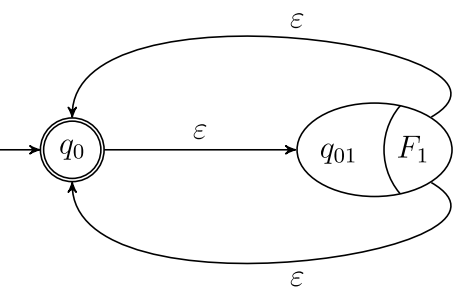
\includegraphics[width=0.7\textwidth]{Blatt10_4.png}
  
  Offenbar ist $\A_\varepsilon$ ein $\varepsilon$-NEA. Mit Lemma 1.12 bekommt man einen zu $\A_\varepsilon$ äquivalenten NEA, nennen wir ihn $\A_{\text{NEA}}$. Äquivalent bedeutet $L(\A_\varepsilon)=\A_{\text{NEA}}$.\nl
  Bleibt noch zu zeigen, dass $L(\A_\varepsilon)=L^\ast$ gilt. 
  Sei also $w\in L^\ast$.
  Dann gibt es ein $n\in\N$ so, dass $w\in\bigcup\limits_{i=1}^n L$ ist. Man sieht leicht, dass $w\in L(\A_\varepsilon)$ liegen muss. (Das formal aufzuschreiben ist ein wenig sperrig.)
\end{proof}

\section*{Aufgabe 5}
Beweis oder Widerlege:
\begin{enumerate}[label=\alph*)]
	\item $L$ erkennbar $\implies\exists\varepsilon$-NEA $\A:L(\A)=L$.\\
	Stimmt, denn:
	\begin{align*}
		L\text{ erkennbar}
		\overset{\text{Def 1.6}}&\implies
		\exists\text{NEA}\A_N:L(\A_N)=L\\
		\overset{\text{Lemma 10}}&\implies
		\exists\varepsilon\text{-NEA }\A:L(\A)\overset{\text{Def 1.6}}{=}L(\A_N)=L
	\end{align*}
	\item $\exists$ NEA mit Wortübergängen mit $L(\A)=L\implies L$ erkennbar.\\
	Stimmt, denn:
	\begin{align*}
		&\exists\text{ NEA $\A$ mit Wortübergängen mit }L(\A)=L\\
		\overset{\text{Satz 1.9}}&\implies
		\exists\text{ NEA }\A_N:L(\A_N)\overset{\text{Def 1.6}}=L(\A)=L\\
		\overset{\text{Def 1.6}}&\implies
		L\text{ erkennbar}
	\end{align*}
	\item $\exists$ Transitionssystem $\A$ mit $L(\A)=L\implies L$ erkennbar\\
	Das stimmt nicht, denn man betrachte ein Transitionssystem mit $Q=\infty$, z. B.
	\begin{align*}
		\A:=\Big(\N_{\geq0},\lbrace a\rbrace,\lbrace0\rbrace,\Delta:=\lbrace(q_i,a,q_{i+1})\mid i\in\N_{\geq0}\rbrace,F:=\N\Big)
	\end{align*}
	Dann gilt
	\begin{align*}
		a^\infty\in L(\A)
	\end{align*}
	Hm... irgendwie ist das wohl doch nicht ganz richtig %TODO
	\item $L$ erkennbar und $L\subseteq L'\implies L'$ erkennbar\\
	Stimmt nicht.
	%TODO
	\item $L$ erkennbar und $L'\subseteq L\implies L'$ erkennbar.\\
	Stimmt. %TODO
	\item $L_1,L_2$ erkennbar $\implies L:=L_1\cap L_2$ erkennbar.\\
	Stimmt, wegen Satz 4.1
	\item Wenn es ein $n\in\N$ gibt, so dass $\cong_L$ (Nerode-Rechtskongruenz) höchstens $n$ Äquivalenzklassen hat, so ist $L$ erkennbar.\\
	%TODO
	
\end{enumerate}

\end{document}